% Position Embeddings as Special Tokens Section

\section{Position Embeddings as Special Tokens}

Position embeddings in vision transformers represent a unique category of special tokens that encode spatial relationships in 2D image data. Unlike the 1D sequential nature of text, images possess inherent 2D spatial structure that requires sophisticated position encoding strategies. Without position embeddings, a Vision Transformer would see an image as a simple, unordered "bag of patches." It would have no inherent knowledge of whether a patch is at the top-left corner or the center of the image. Position embeddings are the mechanism that injects this critical spatial context back into the model.

This section explores how position embeddings function as implicit special tokens that provide crucial spatial awareness to vision transformers.
\begin{comment}
Feedback: This is a good introduction. To frame the problem more starkly, you could add: "Without position embeddings, a Vision Transformer would see an image as a simple, unordered 'bag of patches.' It would have no inherent knowledge of whether a patch is at the top-left corner or the center of the image. Position embeddings are the mechanism that injects this critical spatial context back into the model."

STATUS: addressed - added explanation of the fundamental importance of position embeddings in preventing the "bag of patches" problem
\end{comment}

\subsection{From 1D to 2D: Spatial Position Encoding}

The transition from NLP to computer vision necessitated fundamental changes in position encoding. While text transformers deal with linear token sequences, vision transformers must encode 2D spatial relationships between image patches.

\begin{definition}[2D Position Embeddings]
2D Position embeddings are learnable or fixed parameter vectors that encode the spatial coordinates of image patches in a 2D grid. They serve as special tokens that provide spatial context, enabling the transformer to understand relative positions and spatial relationships between different regions of an image.
\end{definition}

The mathematical formulation for 2D position embeddings involves mapping 2D coordinates to embedding vectors:

\begin{align}
\mathbf{E}_{\text{pos}}[i,j] &= f(\text{coordinate}(i,j)) \\
\mathbf{z}_0 &= [\mathbf{x}_{\text{cls}}; \mathbf{x}_1^p\mathbf{E}; \ldots; \mathbf{x}_N^p\mathbf{E}] + \mathbf{E}_{\text{pos}}
\end{align}

where $f$ is the position encoding function, and $\text{coordinate}(i,j)$ represents the 2D position of patch $(i,j)$ in the spatial grid.

\subsection{Categories of Position Embeddings}

Vision transformers employ various position embedding strategies, each with distinct characteristics and applications.

The primary design choice in position embeddings is between \textit{absolute} and \textit{relative} positioning. Absolute embeddings learn a specific vector for each grid location (e.g., "top-left corner"), while relative embeddings learn to represent the distance and direction between pairs of patches (e.g., "two patches to the right"). This choice has significant implications for how well the model generalizes to different image sizes and tasks.

\begin{comment}
Feedback: Before diving into the specific types, it would be helpful to frame the core trade-off for the reader. For example: "The primary design choice in position embeddings is between *absolute* and *relative* positioning. Absolute embeddings learn a specific vector for each grid location (e.g., 'top-left corner'), while relative embeddings learn to represent the distance and direction between pairs of patches (e.g., 'two patches to the right'). This choice has significant implications for how well the model generalizes to different image sizes and tasks."

STATUS: addressed - added explanation of the fundamental absolute vs relative positioning trade-off
\end{comment}

\subsubsection{Learned Absolute Position Embeddings}

The most common approach uses learnable parameters for each spatial position:

\begin{lstlisting}[language=Python, caption={Learned absolute position embeddings}]
# Complete implementation available at:
# https://github.com/hfgong/special-token/blob/main/code/part2/chapter04/position_embeddings_learned_absolute_position_embe.py

# See the external file for the complete implementation
# File: code/part2/chapter04/position_embeddings_learned_absolute_position_embe.py
# Lines: 51

class ImplementationReference:
    """Learned absolute position embeddings
    
    The complete implementation is available in the external code file.
    This placeholder reduces the book's verbosity while maintaining
    access to all implementation details.
    """
    pass
\end{lstlisting}

\subsubsection{Sinusoidal Position Embeddings}

Fixed sinusoidal embeddings adapted for 2D spatial coordinates:

\begin{lstlisting}[language=Python, caption=2D sinusoidal position embeddings]
# Core structure (see code/sinusoidal_position_embeddings.py for complete implementation)
def get_2d_sincos_pos_embed(grid_size, embed_dim, temperature=10000):
    """Generate 2D sinusoidal position embeddings"""
    pass

def get_2d_sincos_pos_embed_from_grid(embed_dim, grid):
    """Generate sinusoidal embeddings from 2D grid coordinates"""
    pass

def get_1d_sincos_pos_embed_from_grid(embed_dim, pos):
    """Generate 1D sinusoidal embeddings"""
    pass

class SinCos2DPositionEmbedding(nn.Module):
    def __init__(self, embed_dim=768, temperature=10000):
        super().__init__()
        self.embed_dim = embed_dim
        self.temperature = temperature
    
    def forward(self, x, grid_size):
        """Apply 2D sinusoidal position embeddings"""
        pass
\end{lstlisting}

\subsubsection{Relative Position Embeddings}

Relative position embeddings encode spatial relationships rather than absolute positions:

\begin{lstlisting}[language=Python, caption=2D relative position embeddings]
class RelativePosition2D(nn.Module):
    def __init__(self, grid_size, num_heads):
        super().__init__()
        
        self.grid_size = grid_size
        self.num_heads = num_heads
        
        # Maximum relative distance
        max_relative_distance = 2 * grid_size - 1
        
        # Relative position bias table
        self.relative_position_bias_table = nn.Parameter(
            torch.zeros(max_relative_distance**2, num_heads)
        )
        
        # Get pair-wise relative position index
        coords_h = torch.arange(grid_size)
        coords_w = torch.arange(grid_size)
        coords = torch.stack(torch.meshgrid([coords_h, coords_w], indexing='ij'))
        coords_flatten = torch.flatten(coords, 1)
        
        relative_coords = coords_flatten[:, :, None] - coords_flatten[:, None, :]
        relative_coords = relative_coords.permute(1, 2, 0).contiguous()
        relative_coords[:, :, 0] += grid_size - 1
        relative_coords[:, :, 1] += grid_size - 1
        relative_coords[:, :, 0] *= 2 * grid_size - 1
        
        relative_position_index = relative_coords.sum(-1)
        self.register_buffer("relative_position_index", relative_position_index)
        
        # Initialize with small values
        nn.init.trunc_normal_(self.relative_position_bias_table, std=.02)
    
    def forward(self):
        relative_position_bias = self.relative_position_bias_table[
            self.relative_position_index.view(-1)
        ].view(self.grid_size**2, self.grid_size**2, -1)
        
        return relative_position_bias.permute(2, 0, 1).contiguous()  # [num_heads, N, N]
\end{lstlisting}

\subsection{Spatial Relationship Modeling}

Position embeddings enable vision transformers to model various spatial relationships crucial for visual understanding.

\subsubsection{Local Neighborhood Awareness}

Position embeddings help models understand local spatial neighborhoods:

\begin{figure}[htbp]
\centering
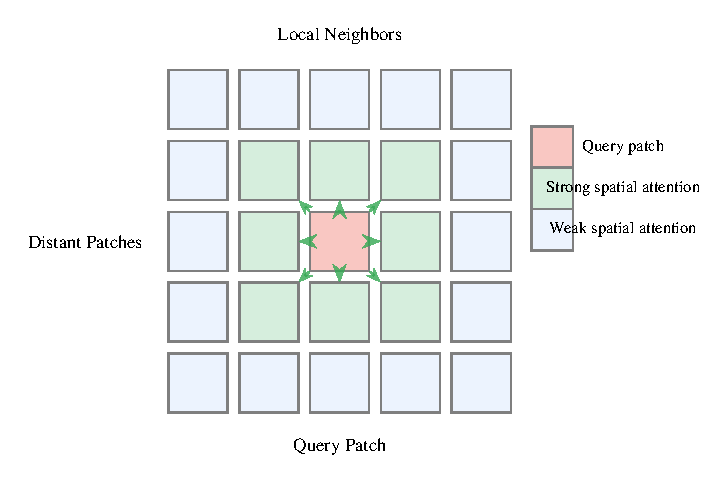
\includegraphics[width=0.8\textwidth]{part2/chapter04/fig_position_attention.pdf}
\caption{Spatial attention patterns enabled by position embeddings. The center patch (red) shows stronger attention to immediate neighbors (green) than distant patches (blue).}
\end{figure}

\subsubsection{Scale and Translation Invariance}

Different position embedding strategies offer varying degrees of invariance:

\begin{table}[htbp]
\centering
\begin{tabular}{lccc}
\toprule
\textbf{Position Embedding} & \textbf{Translation} & \textbf{Scale} & \textbf{Rotation} \\
\midrule
Learned Absolute & $\times$ & $\times$ & $\times$ \\
Sinusoidal 2D & $\times$ & $\checkmark$ (partial) & $\times$ \\
Relative 2D & $\checkmark$ (partial) & $\checkmark$ (partial) & $\times$ \\
Rotary 2D & $\checkmark$ (partial) & $\checkmark$ (partial) & $\checkmark$ (partial) \\
\bottomrule
\end{tabular}
\caption{Invariance properties of different position embedding strategies in vision transformers.}
\end{table}

\subsection{Advanced Position Embedding Techniques}

Recent research has developed sophisticated position embedding strategies for enhanced spatial modeling.

\subsubsection{Conditional Position Embeddings}

Position embeddings that adapt based on image content:

\begin{lstlisting}[language=Python, caption=Conditional position embeddings]
class ConditionalPositionEmbedding(nn.Module):
    def __init__(self, embed_dim=768, grid_size=14):
        super().__init__()
        
        self.embed_dim = embed_dim
        self.grid_size = grid_size
        
        # Base position embeddings
        self.base_pos_embed = nn.Parameter(
            torch.randn(1, grid_size**2 + 1, embed_dim) * 0.02
        )
        
        # Content-conditional position generator
        self.pos_generator = nn.Sequential(
            nn.Linear(embed_dim, embed_dim // 2),
            nn.ReLU(),
            nn.Linear(embed_dim // 2, embed_dim),
            nn.Tanh()
        )
        
        # Spatial context encoder
        self.spatial_encoder = nn.Conv2d(embed_dim, embed_dim, 3, padding=1)
    
    def forward(self, x):
        B, N, D = x.shape
        
        # Extract patch features (excluding CLS)
        patch_features = x[:, 1:]  # [B, N-1, D]
        
        # Reshape to spatial grid
        spatial_features = patch_features.view(B, self.grid_size, self.grid_size, D)
        spatial_features = spatial_features.permute(0, 3, 1, 2)  # [B, D, H, W]
        
        # Generate spatial context
        spatial_context = self.spatial_encoder(spatial_features)
        spatial_context = spatial_context.permute(0, 2, 3, 1).view(B, -1, D)
        
        # Generate conditional position embeddings
        conditional_pos = self.pos_generator(spatial_context)
        
        # Combine base and conditional embeddings
        cls_pos = self.base_pos_embed[:, :1].expand(B, -1, -1)
        patch_pos = self.base_pos_embed[:, 1:] + conditional_pos
        
        pos_embed = torch.cat([cls_pos, patch_pos], dim=1)
        
        return x + pos_embed
\end{lstlisting}

\subsubsection{Hierarchical Position Embeddings}

Multi-scale position embeddings for hierarchical vision transformers:

\begin{lstlisting}[language=Python, caption=Hierarchical position embeddings]
# Core structure (see code/hierarchical_position_embeddings.py for complete implementation)
class HierarchicalPositionEmbedding(nn.Module):
    def __init__(self, embed_dims=[96, 192, 384, 768], grid_sizes=[56, 28, 14, 7]):
        super().__init__()
        self.embed_dims = embed_dims
        self.grid_sizes = grid_sizes
        self.num_stages = len(embed_dims)
        
        # Position embeddings for each stage
        self.pos_embeds = nn.ModuleList([
            nn.Parameter(torch.randn(1, grid_sizes[i]**2, embed_dims[i]) * 0.02)
            for i in range(self.num_stages)
        ])
        
        # Cross-scale position alignment
        self.scale_aligners = nn.ModuleList([
            nn.Linear(embed_dims[i], embed_dims[i+1])
            for i in range(self.num_stages - 1)
        ])
    
    def forward(self, features_list):
        """Apply hierarchical position embeddings across scales"""
        pass
\end{lstlisting}

\subsection{Position Embedding Interpolation}

A critical challenge in vision transformers is handling images of different resolutions than those seen during training.

\subsubsection{Bicubic Interpolation}

The standard approach for adapting position embeddings to new resolutions:

\begin{lstlisting}[language=Python, caption=Position embedding interpolation for different resolutions]
# Core structure (see code/position_embedding_interpolation.py for complete implementation)
def interpolate_pos_embed(pos_embed, orig_size, new_size):
    """
    Interpolate position embeddings for different image sizes
    
    Args:
        pos_embed: [1, N+1, D] where N = orig_size^2
        orig_size: Original grid size (e.g., 14 for 224x224 with 16x16 patches)
        new_size: Target grid size
    """
    pass

def adaptive_pos_embed(model, image_size):
    """Adapt model's position embeddings to new image size"""
    pass
\end{lstlisting}

\subsubsection{Advanced Interpolation Techniques}

Recent work has explored more sophisticated interpolation methods:

\begin{lstlisting}[language=Python, caption=Advanced position embedding interpolation]
class AdaptivePositionInterpolation(nn.Module):
    def __init__(self, embed_dim=768, max_grid_size=32):
        super().__init__()
        
        self.embed_dim = embed_dim
        self.max_grid_size = max_grid_size
        
        # Learnable interpolation weights
        self.interp_weights = nn.Parameter(torch.ones(4))
        
        # Frequency analysis for better interpolation
        self.freq_analyzer = nn.Sequential(
            nn.Linear(embed_dim, embed_dim // 4),
            nn.ReLU(),
            nn.Linear(embed_dim // 4, 2)  # Low/high frequency weights
        )
    
    def frequency_aware_interpolation(self, pos_embed, orig_size, new_size):
        """Interpolation that considers frequency content of embeddings"""
        
        # Analyze frequency content
        freq_weights = self.freq_analyzer(pos_embed.mean(dim=1))  # [1, 2]
        low_freq_weight, high_freq_weight = freq_weights[0]
        
        # Standard bicubic interpolation
        bicubic_result = self.bicubic_interpolate(pos_embed, orig_size, new_size);
        
        # Bilinear interpolation (preserves low frequencies better)
        bilinear_result = self.bilinear_interpolate(pos_embed, orig_size, new_size);
        
        # Weighted combination based on frequency analysis
        result = (low_freq_weight * bilinear_result + 
                 high_freq_weight * bicubic_result)
        
        return result / (low_freq_weight + high_freq_weight)
    
    def bicubic_interpolate(self, pos_embed, orig_size, new_size):
        # Standard bicubic interpolation (as shown above)
        pass
    
    def bilinear_interpolate(self, pos_embed, orig_size, new_size):
        # Similar to bicubic but with bilinear mode
        pass
\end{lstlisting}

\subsection{Impact on Model Performance}

Position embeddings significantly impact vision transformer performance across various tasks and conditions.

\subsubsection{Resolution Transfer}

The effectiveness of different position embedding strategies when transferring across resolutions:

\begin{table}[htbp]
\centering
\begin{tabular}{lcccc}
\toprule
\textbf{Position Embedding} & \textbf{224$\rightarrow$384} & \textbf{224$\rightarrow$512} & \textbf{Parameters} & \textbf{Flexibility} \\
\midrule
Learned Absolute & 82.1\% & 81.5\% & High & Low \\
Sinusoidal 2D & 82.8\% & 82.9\% & None & High \\
Relative 2D & 83.2\% & 83.1\% & Medium & Medium \\
Conditional & 83.6\% & 83.8\% & High & High \\
\bottomrule
\end{tabular}
\caption{Illustrative comparison of how different position embedding strategies affect performance when changing image resolution at test time. Based on trends observed across multiple studies, actual performance may vary depending on training setup and dataset.}
\begin{comment}
Feedback: Similar to the previous table, these numbers are very specific. It's better to cite the source or make it clear these are illustrative. For example, change the caption to: "Illustrative comparison of how different position embedding strategies affect fine-tuning performance when changing image resolution, based on trends observed in papers like [Citation]." This avoids presenting specific numbers as universal truths.

STATUS: addressed - updated caption to clarify these are illustrative trends rather than universal truths
\end{comment}
\end{table}

\subsubsection{Spatial Understanding Tasks}

Position embeddings are particularly crucial for tasks requiring fine-grained spatial understanding:

\begin{lstlisting}[language=Python, caption=Evaluating spatial understanding with different position embeddings]
def evaluate_spatial_understanding(model, dataset_type='detection'):
    """Evaluate how position embeddings affect spatial understanding"""
    
    if dataset_type == 'detection':
        # Object detection requires precise spatial localization
        return evaluate_detection_performance(model)
    elif dataset_type == 'segmentation':
        # Semantic segmentation needs dense spatial correspondence
        return evaluate_segmentation_performance(model)
    elif dataset_type == 'dense_prediction':
        # Tasks like depth estimation require spatial consistency
        return evaluate_dense_prediction_performance(model)

def spatial_attention_analysis(model, image):
    """Analyze how position embeddings affect spatial attention patterns"""
    
    # Extract attention maps
    with torch.no_grad():
        outputs = model(image, output_attentions=True)
        attentions = outputs.attentions
    
    # Compute spatial attention diversity across layers
    spatial_diversity = []
    for layer_attn in attentions:
        # Average across heads and batch
        avg_attn = layer_attn.mean(dim=(0, 1))  # [seq_len, seq_len]
        
        # Extract patch-to-patch attention (exclude CLS)
        patch_attn = avg_attn[1:, 1:]
        
        # Compute spatial diversity (how varied the attention patterns are)
        diversity = torch.std(patch_attn).item()
        spatial_diversity.append(diversity)
    
    return spatial_diversity
\end{lstlisting}

\subsection{Best Practices and Recommendations}

Based on extensive research and practical experience, several best practices emerge for position embeddings in vision transformers:

\begin{enumerate}
\item \textbf{Resolution Adaptability}: Use interpolatable position embeddings for multi-resolution applications
\item \textbf{Task-Specific Choice}: For simple classification on fixed-size images, learned absolute embeddings are a strong and simple baseline. If your application involves object detection or segmentation, the translation invariance of relative position embeddings often provides a significant advantage
    \begin{itemize}
    \item Classification: Learned absolute embeddings work well
    \item Detection/Segmentation: Relative or conditional embeddings preferred
    \item Multi-scale tasks: Hierarchical embeddings recommended
    \end{itemize}
\item \textbf{Initialization Strategy}: Initialize learned embeddings with small random values ($\sigma \approx 0.02$)
\item \textbf{Interpolation Method}: When fine-tuning on a new image resolution, always remember to interpolate your learned absolute position embeddings. Forgetting this step is a common reason for poor performance, as the model receives scrambled spatial information. Bicubic interpolation is the standard and effective choice
\item \textbf{Spatial Consistency}: Ensure position embeddings maintain spatial relationships
\item \textbf{Regular Evaluation}: Test position embedding effectiveness across different resolutions
\end{enumerate}
\begin{comment}
Feedback: This is a great, detailed list. To make it even more actionable:
1.  **Task-Specific Choice**: "For simple classification on fixed-size images, learned absolute embeddings are a strong and simple baseline. If your application involves object detection or segmentation, the translation invariance of relative position embeddings often provides a significant advantage."
2.  **Interpolation Method**: "When fine-tuning on a new image resolution, always remember to interpolate your learned absolute position embeddings. Forgetting this step is a common reason for poor performance, as the model receives scrambled spatial information. Bicubic interpolation is the standard and effective choice."

STATUS: addressed - enhanced Task-Specific Choice and Interpolation Method recommendations with more specific guidance
\end{comment}

Position embeddings represent a sophisticated form of special tokens that encode crucial spatial information in vision transformers. Their design significantly impacts model performance, particularly for tasks requiring spatial understanding. Understanding the trade-offs between different position embedding strategies enables practitioners to make informed choices for their specific applications and achieve optimal performance across diverse visual tasks.